\documentclass[aspectratio=169,dvipsnames]{beamer}

%\usepackage[czech]{babel}
\usepackage[nounicodemath,custombib,czech]{ufalslides}
\usepackage{xcolor}
\usepackage{textcomp}
\usepackage{booktabs}
\usepackage{collcell}
\usepackage{xstring}
\usepackage{tikz-dependency}

\usepackage{csquotes}
\usepackage[citestyle=authoryear]{biblatex}


\makeatletter
\def\blx@nowarnpolyglossia{1}
\makeatother

\bibliography{odkazy.bib}

\usepackage{tikz}
\usepackage{gnuplot-lua-tikz}
\usepackage{tikz-qtree}
\usetikzlibrary{calc}
\usetikzlibrary{arrows,shapes,positioning}
\usetikzlibrary{arrows.meta}

\setbeamercolor{blockcolor}{bg=gray!20, fg=black}


% %%%%%%%%%%%%%%%%%%%%%%%%%%%%%%%%%%%%%%%%%%%%%%%%%%%%%%%%%%%%%%%%%%%%%%%%%%%%%
\def\course{NAIL127 AI v Kontextu}
\def\courseurl{https://ufal.mff.cuni.cz/AIvK}
\def\title{Úvodní přednáška}
\def\subtitle{Co je a není AI, co je strojové učení a neuronové sítě}
\def\author{Jindřich Libovický, Tereza Hanemann, Rudolf Rosa}
\def\date{14. února 2022}
\def\licence{cc-by-nc-sa}
%\def\langtech{}
\def\shownavigation{}
% %%%%%%%%%%%%%%%%%%%%%%%%%%%%%%%%%%%%%%%%%%%%%%%%%%%%%%%%%%%%%%%%%%%%%%%%%%%%%

\begin{document}

\maketitle

\section{AI v Kontextu}

\begin{frame}{Tým AI v kontextu}

    \begin{columns}
        \column{30pt}
    \begin{tikzpicture}
    \clip (0,0) circle (30pt);
    \node at (0.0,-0.15) {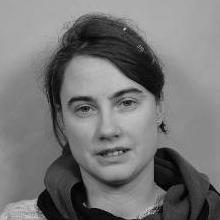
\includegraphics[scale=0.3]{img/tereza.jpg}};
    \end{tikzpicture}
        \column{.6\textwidth}
        \textbf{Tereza Hanemann}

    \end{columns}

    \hspace*{20pt}\begin{columns}
        \column{30pt}
    \begin{tikzpicture}
    \clip (0,0) circle (30pt);
    \node at (0.0,-0.7) {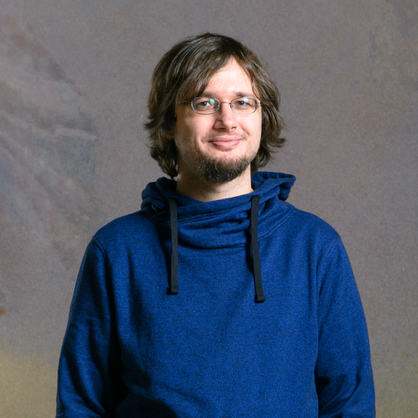
\includegraphics[scale=0.35]{img/rudolfrosa.png}};
    \end{tikzpicture}
        \column{.6\textwidth}
        \textbf{Rudolf Rosa}

    \end{columns}

    \hspace*{40pt}\begin{columns}
        \column{30pt}
    \begin{tikzpicture}
    \clip (0,0) circle (30pt);
    \node at (0.0,-0.3) {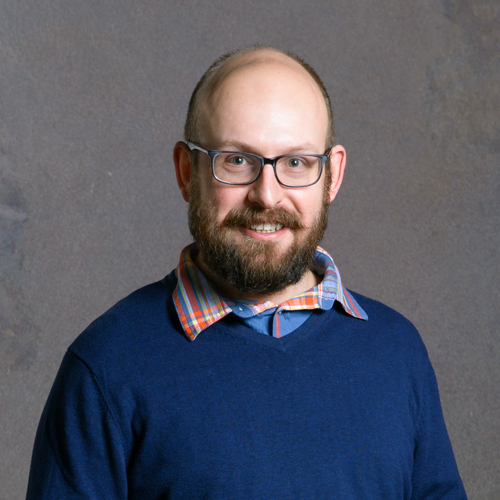
\includegraphics[scale=0.35]{img/jindrich.jpg}};
    \end{tikzpicture}
        \column{.6\textwidth}
        \textbf{Jindřich Libovický}

    \end{columns}

\end{frame}

% ----------------------------------------------------------------------------

\begin{frame}{Organizace předmětu}
\end{frame}
% ----------------------------------------------------------------------------

\begin{frame}{Program}
\end{frame}

\section{Co je umělá inteligence}

% ----------------------------------------------------------------------------

\begin{frame}{Ne-definice}

    \begin{center}
        \Large
    \textbf{Umělá inteligence} = obor informatiky, který se zabývá řešením
    úloh\ldots
    \end{center}

    \vspace{10pt}

    \begin{itemize}

        \item<2-> O kterých se vágně shodneme, že k~jejich řešení lidé potřebují
            inteligenci

        \item<3-> Někdy úlohy, které vyžadují \textbf{velké mentální úsilí} \\
            \quad \emph{hraní šachů nebo Go, automatický překlad}

        \item<4-> Někdy úlohy, které jsou \textbf{pro člověka triviální} \\
            \quad \emph{rozpoznávání objektů na fotografii, rozpozávání řeči}

    \end{itemize}

    \centering\vspace{15pt}

    \visible<5->{Hranice, co je a není AI, se posouvá\ldots}

\end{frame}

% ----------------------------------------------------------------------------

\begin{frame}{Inteligentní chování = AI?}

    \begin{columns}
        \column{.40\textwidth}
        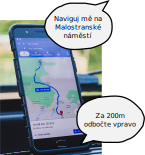
\includegraphics[scale=0.45]{./img/navigation.pdf}

        \column{.55\textwidth}

        \begin{enumerate}

            \item<2-> Rozpoznávání řeči \\
                \visible<9->{\hfill\it\color{gray} neuronová síť naučená z nahrávek}

            \item<3-> Analýza textu \\
                \visible<10->{\hfill\it\color{gray} pravidla nebo neuronová síť}

            \item<4-> Vyhledání cíle na mapě \\
                \visible<11->{\hfill\it\color{gray} vyhledávání v databázi, spíš SW inženýrství}

            \item<5-> Nalezení nejlepší cesty \\
                \visible<12->{\hfill\it\color{gray} optimalizace, diskrétní matematika}

            \item<6-> Určení polohy, rozhodnutí co je další krok na nejlepší cestě
                \visible<13->{\hfill\it\color{gray} jednoduchý algoritmus}

            \item<7-> Generování přirozeného jazyka \\
                \visible<14->{\hfill\it\color{gray} jednoduchý algoritmus nebo neuronová síť}

            \item<8-> Syntéza řeči \\
                \visible<15->{\hfill\it\color{gray} neuronová síť naučená z nahrávek}

        \end{itemize}

    \end{columns}

\end{frame}

% ----------------------------------------------------------------------------

\begin{frame}{Strong vs. Weak AI}

    \begin{columns}[t]
        \column{.45\textwidth}
        \visible<1->{{\large \textbf{Strong AI}}}

        \vspace{5pt}

        \begin{itemize}

            \item<2-> Také AGI -- Artifitial General Inteligence

            \item<3-> Cílem je obecně \textbf{inteligentní stroj}, který v důsledku
                toho umí řešit úlohy

            \item<4-> Zajímavé filozofické problémy: Inteligenční singularita?
                Musela by být AGI vtělená?

        \end{itemize}


        \column{.45\textwidth}
        \visible<5->{{\large \textbf{Weak AI}}}

        \vspace{5pt}

        \begin{itemize}

            \item<6-> Také Narrow AI

            \item<7-> Cílem je řešit \textbf{jednotlivé úlohy}, které vyžadují
                inteligenci

            \item<8-> Všechno, o čem bude řeč, je weak AI

        \end{itemize}
    \end{columns}


\end{frame}

% ----------------------------------------------------------------------------

\begin{frame}{Strong AI: Turingův test}

\end{frame}

% ----------------------------------------------------------------------------

\begin{frame}{Strong AI: Čínský pokoj}

\end{frame}

% ----------------------------------------------------------------------------

\begin{frame}{Když se dneska řekne AI}

    \Large

    \begin{itemize}

        \item Myslí se \textbf{weak AI}

        \item Většinou jsou to metody založené na strojovém učení a zpracování
            hodně dat

        \item Často je to strojové učení pomocí neuronových sítí

    \end{itemize}


\end{frame}


% ----------------------------------------------------------------------------

\section{Strojové učení \& Neuronové sítě}

\begin{frame}{Běžné programování vs.\ strojové učení}

    {\large \textbf{Programování řešení}}

    \begin{itemize}

        \item<2-> Jsme schopni problém \textbf{formálně popsat} jasnými koncepty

        \item<3-> Program je jednoznačný návod, jak s koncepty zacházet

    \end{itemize}

    \vspace{10pt}

    \visible<3->{%
    \begin{beamercolorbox}{blockcolor}
    {\color{ufal} Příklad -- E-shop:} {\it Koncepty: zboží, sklad, zákazník,
    objednávka} \\
    \quad Udělat obědnávku, odeslat obědnávku = jednoduchý algoritmus
    \end{beamercolorbox}}

    \vspace{20pt}

    \visible<4->{{\large \textbf{Učení řešení}}}

    \begin{itemize}

        \item<5-> Máme \textbf{příklady} vstupů a výstupů

        \item<6-> Nejsme schopni do důsledku napsat návod, jak úlohu řešit

    \end{itemize}

    \vspace{10pt}

    \visible<7->{%
    \begin{beamercolorbox}[]{blockcolor}
    {\color{ufal} Příklad -- strojový překlad:} {\it neexstiuje návod, pro člověka, který nerozumím oběma jazykům} \\
    \quad Existuje mnoho přeložených textů, co se dají použít pro trénování
    \end{beamercolorbox}}

\end{frame}

% ----------------------------------------------------------------------------

\begin{frame}{Obecné schéma}

    \centering
\scalebox{.8}{%
\begin{tikzpicture}%
[   normal arrow/.style={draw,-triangle 45,very thick},
    big box/.style={draw=####1!20!black, fill=####1!60, minimum width=9em, minimum height=9em, rectangle, align=center},
    small box/.style={draw, minimum height=5mm, minimum width=####1, rectangle}
]
\node[big box = RoyalBlue] (d) at (1, -5) {};
\node[above] at (d.north) {};
\node[below, align=center] at (d.north) {data};
\node[big box = ForestGreen] (a) at (7, -5) {};
\node[below, align=center] at (a.north) {učící algoritmus};
\node[big box = Dandelion] (m) at (14, -5) {};
\node[below, align=center] at (m.north) {model};

\path[normal arrow] (d) -- (a);
\path[normal arrow] (a) -- (m);

\foreach \x in {1,...,3} {%
	\node[small box = 5em] (x\x) at (0.4, -3.4 - \x * 0.8) {$x_{\x}$};
	\node[small box = 1.5em] (y\x) at (2.2, -3.4 - \x * 0.8) {$y_{\x}$};
	\path[draw] (x\x) -- (y\x);
}
\node[] (xc) at (0.4, -3.2 - 4 * 0.8) {$\vdots$};
\node[] (yc) at (2.2, -3.2 - 4 * 0.8) {$\vdots$};

\node[small box = 5em] (x) at (14, -2) {$x$};
\node[small box = 1.5em] (y) at (14, -8) {$y$};

\path[normal arrow] (x) -- (m);
\path[normal arrow] (m) -- (y);

\node[] (p) at (7, -1.5) {předpoklady};
\node[] (po) at (7, -8.5) {požadavky};

\path[draw, triangle 45-triangle 45, dashed] (d) -- (p);
\path[normal arrow] (p) -- (a);
\path[draw, triangle 45-triangle 45, dashed] (po) -- (m);
\path[normal arrow] (po) -- (a);

\node[small box = 6em] (meta) at (7, -5) {metaparametry};

\node[small box = 6em] (par-alg) at (14, -5) {algoritmus};
\node[small box = 6em] (par) at (14, -6) {parametry};

\end{tikzpicture}}
\end{frame}

\begin{frame}{Příklad: klasifikace obrázků}
\end{frame}

\begin{frame}{Generalizace vs. přeučení}
\end{frame}

\begin{frame}{Neuronové síťě}
Neuronony nejsou ani náhodou biologické neurony

Nějaká historie
\end{frame}

\begin{frame}{Neuronová síť}
Jak vypadá jednoduchá neuronová síť
Je to vlastně spojitá funkce, co má hodně parameterů
\end{frame}

% ----------------------------------------------------------------------------

\begin{frame}{Chybová funkce}
\end{frame}

% ----------------------------------------------------------------------------

\begin{frame}{Trénování}
\end{frame}

% ----------------------------------------------------------------------------

\begin{frame}{Kde se berou trénovací data}

    {\large\textbf{Stahování z internetu}} --- neprezentativní, extrémní názory
    jsou mnohem víc slyšet, není kontrola nad tím, co je v datech

    {\large\textbf{Crowd-sourcing}} --- využívání levné pracovní síly, vznikají
    prekarizovaná zaměstnání

    {\large\textbf{Vytěžování existujících databází}} --- 

\end{frame}

% ----------------------------------------------------------------------------

\begin{frame}{Rizika učení z dat}
Učí se z dat -- co je v datech, to je v modelu; chybová funkce (typicky počet správně klasifikovaných příkladů) nemusí postihnout problémy, které model může mít - příklad analýza CV

\end{frame}

\begin{frame}{}
\end{frame}

% ----------------------------------------------------------------------------

\section{Strojové vidění}

\begin{frame}{Úlohy strojového vidění}

    \vspace{-5pt}
    \begin{center}
        \large Cokoli, co se dá zjistit z obrazu, např. \ldots
    \end{center}

    \visible<2->{
    \begin{columns}[t]
        \column{.3\textwidth}
        \centering \textbf{Rozpoznávání objektů} \\[1ex]
        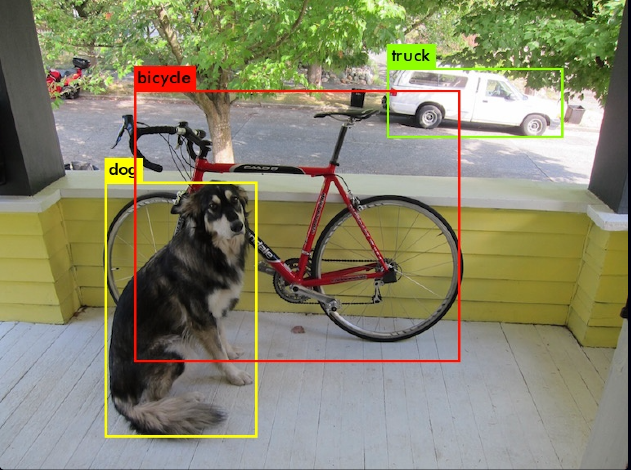
\includegraphics[width=.98\textwidth]{img/object_detection.png} \\
        {\tiny Zdroj: \url{https://pjreddie.com/darknet/yolo}}

        \column{.3\textwidth}
        \centering \textbf{Odhad hloubky v obrazu} \\[1ex]
        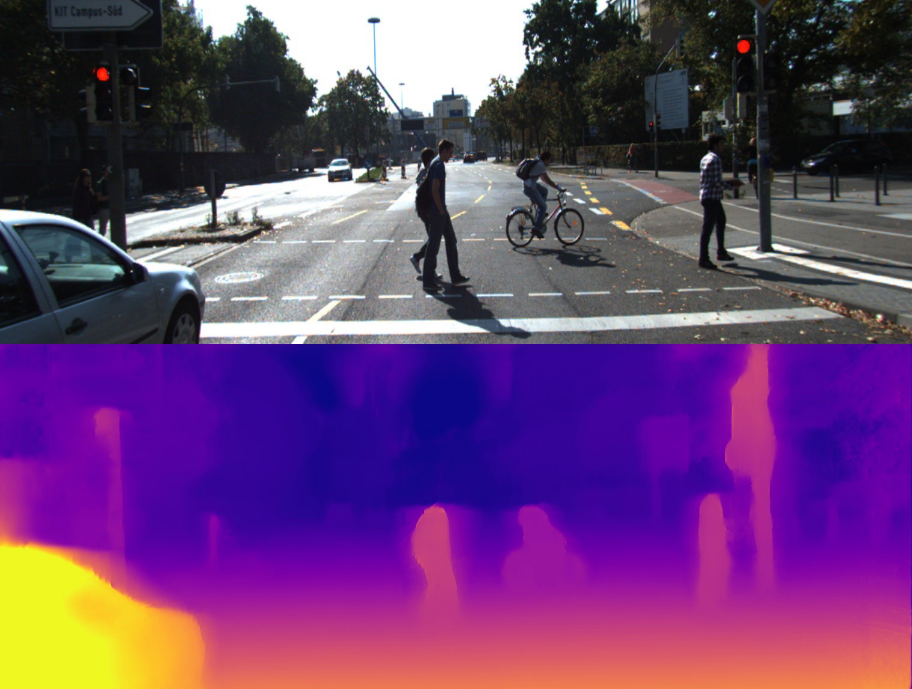
\includegraphics[width=.98\textwidth]{img/monocular_depth.png} \\
        {\tiny Zdroj: \url{https://arxiv.org/abs/1810.01849}}

        \column{.3\textwidth}
        \centering \textbf{Poloha lidského těla} \\[1ex]
        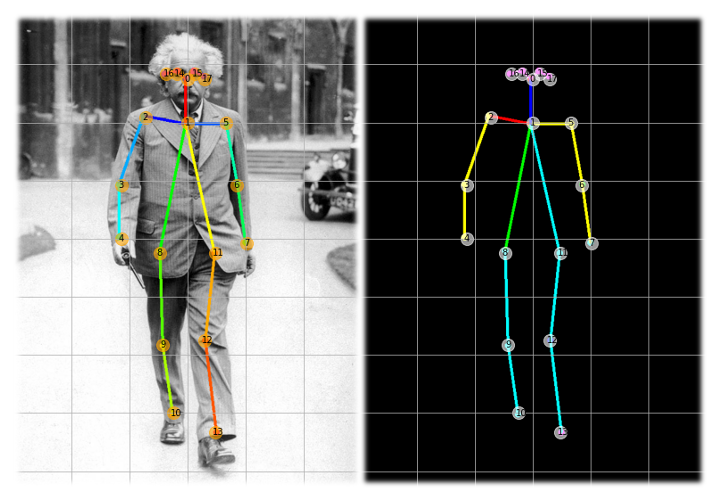
\includegraphics[width=.98\textwidth]{img/pose_detection.png} \\
        {\tiny Zdroj: \url{https://towardsdatascience.com/realtime-multiple-person-2d-pose-estimation-using-tensorflow2-x-93e4c156d45f}}

    \end{columns}}

    \visible<3->{\begin{center}
        \large \ldots pro člověka většinou triviální úlohy
    \end{center}}

\end{frame}

% ----------------------------------------------------------------------------

\begin{frame}{Konvoluční sítě}

    \begin{minipage}{.45\textwidth}
        \begin{itemize}[<+->]

            \item Základní nástroj pro zpracování obrazu neuronovými sítěmi

            \item Okénko, které jede přes obrázek a detekuje nějaké vzorce

            \item Mnoho vrstvev $\rightarrow$ vzorce vzorců vzorců\ldots

            \item Model si vytváří potřebné abstrakce

        \end{itemize}
    \end{minipage}\begin{minipage}{.45\textwidth}
        \centering
        \scalebox{0.7}{\input{img/convolution2d.pdf_tex}}
    \end{minipage}

\end{frame}

% ----------------------------------------------------------------------------

\begin{frame}{Hluboké konvoluční sítě}

    \begin{center}
        \scalebox{0.4}{\input{./img/alexnet.pdf_tex}}
    \end{center}

    \begin{itemize}[<+->]

        \item Architecture: convolutions, max-pooling, residual connections,
            batch normalization, 50--150 layers

        \item Most frequent pre-training: ImageNet --- millions of images, 1k
            labels

    \end{itemize}
ImageNet - předtrénovaná reprezentace z ImageNetu použitelná na jakoukoli jinou úlohu (ukázat úlohy: object detection, monocular depth estimation)
\end{frame}

% ----------------------------------------------------------------------------

\begin{frame}{ImageNet challenge}

    %\begin{tikzpicture}[gnuplot]
%% generated with GNUPLOT 5.2p8 (Lua 5.3; terminal rev. Nov 2018, script rev. 108)
%% Po 31. ledna 2022, 18:45:58
\path (0.000,0.000) rectangle (13.000,7.000);
\gpcolor{color=gp lt color border}
\gpsetlinetype{gp lt border}
\gpsetdashtype{gp dt solid}
\gpsetlinewidth{1.00}
\draw[gp path] (1.504,0.616)--(1.531,0.616);
\draw[gp path] (12.447,0.616)--(12.420,0.616);
\node[gp node right] at (1.320,0.616) {0.00};
\draw[gp path] (1.504,1.629)--(1.531,1.629);
\draw[gp path] (12.447,1.629)--(12.420,1.629);
\node[gp node right] at (1.320,1.629) {0.05};
\draw[gp path] (1.504,2.641)--(1.531,2.641);
\draw[gp path] (12.447,2.641)--(12.420,2.641);
\node[gp node right] at (1.320,2.641) {0.10};
\draw[gp path] (1.504,3.654)--(1.531,3.654);
\draw[gp path] (12.447,3.654)--(12.420,3.654);
\node[gp node right] at (1.320,3.654) {0.15};
\draw[gp path] (1.504,4.666)--(1.531,4.666);
\draw[gp path] (12.447,4.666)--(12.420,4.666);
\node[gp node right] at (1.320,4.666) {0.20};
\draw[gp path] (1.504,5.679)--(1.531,5.679);
\draw[gp path] (12.447,5.679)--(12.420,5.679);
\node[gp node right] at (1.320,5.679) {0.25};
\draw[gp path] (1.504,6.691)--(1.531,6.691);
\draw[gp path] (12.447,6.691)--(12.420,6.691);
\node[gp node right] at (1.320,6.691) {0.30};
\node[gp node center] at (2.572,0.308) {$2011$};
\node[gp node center] at (3.906,0.308) {$2012$};
\node[gp node center] at (5.241,0.308) {$2013$};
\node[gp node center] at (6.575,0.308) {$2014$};
\node[gp node center] at (7.910,0.308) {$2015$};
\node[gp node center] at (9.244,0.308) {$2016$};
\node[gp node center] at (10.579,0.308) {$2017$};
\draw[gp path] (1.504,6.691)--(1.504,0.616)--(12.447,0.616)--(12.447,6.691)--cycle;
\node[gp node center,rotate=-270] at (0.016,3.653) {5-best error rate};
\gpfill{rgb color={0.114,0.188,0.459}} (2.071,0.616)--(3.073,0.616)--(3.073,5.821)--(2.071,5.821)--cycle;
\gpcolor{rgb color={0.114,0.188,0.459}}
\draw[gp path] (2.071,0.616)--(2.071,5.820)--(3.072,5.820)--(3.072,0.616)--cycle;
\gpfill{rgb color={0.114,0.188,0.459}} (3.406,0.616)--(4.408,0.616)--(4.408,3.718)--(3.406,3.718)--cycle;
\draw[gp path] (3.406,0.616)--(3.406,3.717)--(4.407,3.717)--(4.407,0.616)--cycle;
\gpfill{rgb color={0.114,0.188,0.459}} (4.740,0.616)--(5.742,0.616)--(5.742,2.953)--(4.740,2.953)--cycle;
\draw[gp path] (4.740,0.616)--(4.740,2.952)--(5.741,2.952)--(5.741,0.616)--cycle;
\gpfill{rgb color={0.114,0.188,0.459}} (6.075,0.616)--(7.077,0.616)--(7.077,2.117)--(6.075,2.117)--cycle;
\draw[gp path] (6.075,0.616)--(6.075,2.116)--(7.076,2.116)--(7.076,0.616)--cycle;
\gpfill{rgb color={0.114,0.188,0.459}} (7.409,0.616)--(8.411,0.616)--(8.411,1.339)--(7.409,1.339)--cycle;
\draw[gp path] (7.409,0.616)--(7.409,1.338)--(8.410,1.338)--(8.410,0.616)--cycle;
\gpfill{rgb color={0.114,0.188,0.459}} (8.744,0.616)--(9.746,0.616)--(9.746,1.223)--(8.744,1.223)--cycle;
\draw[gp path] (8.744,0.616)--(8.744,1.222)--(9.745,1.222)--(9.745,0.616)--cycle;
\gpfill{rgb color={0.114,0.188,0.459}} (10.078,0.616)--(11.080,0.616)--(11.080,1.073)--(10.078,1.073)--cycle;
\draw[gp path] (10.078,0.616)--(10.078,1.072)--(11.079,1.072)--(11.079,0.616)--cycle;
\gpcolor{color=gp lt color border}
\node[gp node left] at (1.836,6.128) {\footnotesize~err=.257};
\node[gp node left] at (3.170,4.025) {\footnotesize~err=.153};
\node[gp node left] at (4.505,3.260) {\footnotesize~err=.115};
\node[gp node left] at (5.839,2.424) {\footnotesize~err=.074};
\node[gp node left] at (7.174,1.646) {\footnotesize~err=.035};
\node[gp node left] at (8.508,1.530) {\footnotesize~err=.029};
\node[gp node left] at (9.843,1.380) {\footnotesize~err=.022};
\node[gp node left] at (1.836,6.497) {\footnotesize~\citet{sanchez_high-dimensional_2011}};
\node[gp node left] at (3.170,4.394) {\footnotesize~\citet{krizhevsky_imagenet_2012}};
\node[gp node left] at (4.505,3.629) {\footnotesize};
\node[gp node left] at (5.839,2.793) {\footnotesize~\citet{simonyan_very_2014}};
\node[gp node left] at (7.174,2.015) {\footnotesize~\citet{he_deep_2016}};
\node[gp node left] at (8.508,1.899) {\footnotesize};
\node[gp node left] at (9.843,1.749) {\footnotesize~\citet{hu_squeeze-and-excitation_2017}};
\node[gp node left] at (3.170,4.764) {\footnotesize\it~AlexNet};
\node[gp node left] at (5.839,3.163) {\footnotesize\it~VGG19};
\node[gp node left] at (7.174,2.385) {\footnotesize\it~ResNet};
\node[gp node left] at (9.843,2.119) {\scriptsize\it~Squeeze~and~Excitation};
\draw[gp path] (1.504,6.691)--(1.504,0.616)--(12.447,0.616)--(12.447,6.691)--cycle;
%% coordinates of the plot area
\gpdefrectangularnode{gp plot 1}{\pgfpoint{1.504cm}{0.616cm}}{\pgfpoint{12.447cm}{6.691cm}}
\end{tikzpicture}
%% gnuplot variables


\end{frame}


\begin{frame}{Předtrénované reprezentace}
\end{frame}

% ----------------------------------------------------------------------------

\begin{frame}{Problémy ImageNetu}
Problémy imagenetu: koncepty z WordNetu, labely jako “weirdo”, rasistické koncepty…
\end{frame}

% ----------------------------------------------------------------------------

\begin{frame}{Rozpoznávání obličejů}
\end{frame}

% ----------------------------------------------------------------------------

\section{Zpracování přirozeného jazyka}

% ----------------------------------------------------------------------------

\begin{frame}{Co je zpracování přirozeného jazyka}
\end{frame}

% ----------------------------------------------------------------------------

\begin{frame}{Koncept embeddingu}
\end{frame}

% ----------------------------------------------------------------------------

\begin{frame}{Ukázka z překladače}
    \hspace*{-10pt}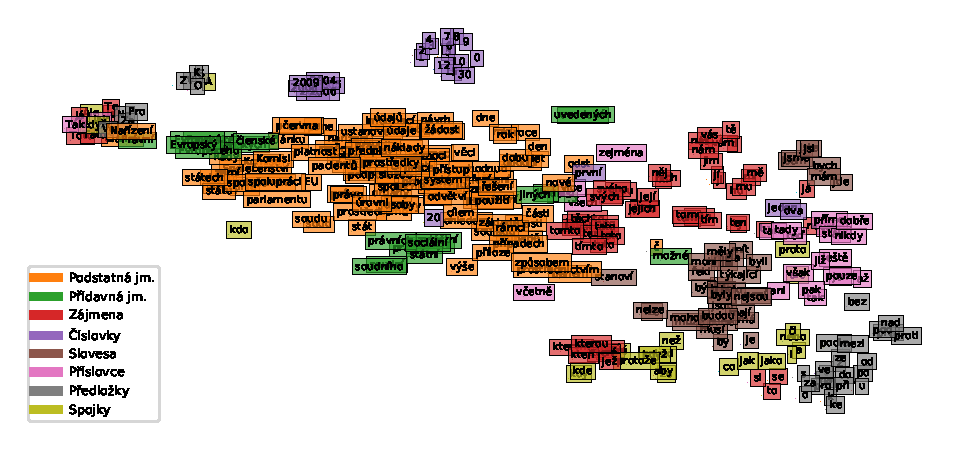
\includegraphics{./plots/tsne.pdf}
\end{frame}

% ----------------------------------------------------------------------------

\begin{frame}{Princip transformeru}
    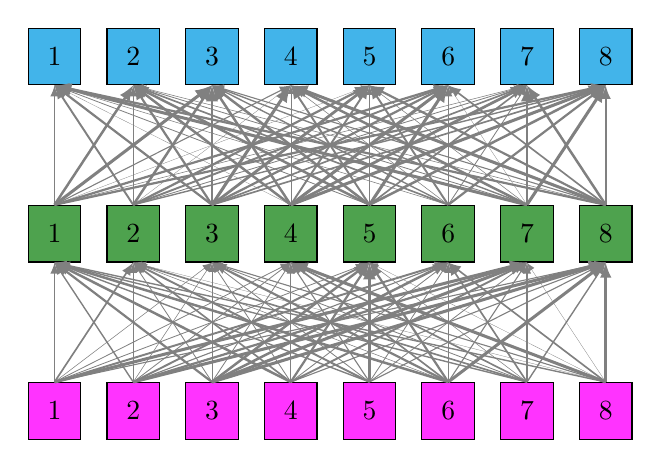
\begin{tikzpicture}

    \foreach \i in {1,...,8}{
			\node[draw,inner sep=7pt,fill=Magenta!80] (A\i) at (\i, 0) {\i};
			\node[draw,inner sep=7pt,fill=ForestGreen!80] (B\i) at (\i, 2.25) {\i};
			\node[draw,inner sep=7pt,fill=Cerulean!80] (C\i) at (\i, 4.5) {\i};
	}

    \foreach \i in {1,...,8}{
		\foreach \j in {1,...,8}{
		    \pgfmathsetmacro{\lnW}{0.1 + random(0,10)/10};
			\draw[->, line width=\lnW, color=Gray, -{latex[width=2mm,length=3mm]}] (A\i.north) -- (B\j.south);
		    \pgfmathsetmacro{\lnW}{0.1 + random(0,10)/10};
			\draw[->, line width=\lnW, color=Gray, -{latex[width=2mm,length=3mm]}] (B\i.north) -- (C\j.south);
		}
	}

\end{tikzpicture}

\end{frame}

% ----------------------------------------------------------------------------

\begin{frame}{Encoder-decoder: Machine translation}
\end{frame}

% ----------------------------------------------------------------------------
\begin{frame}{Zkreslení z dat}
\end{frame}

% ----------------------------------------------------------------------------

\begin{frame}{Předtrénované modely v NLP}

    %málo trénovacích příkladů -- najdi mi všechny tweety, kde se někdo vyjadřuje kritickyo něčemu

    \centering
    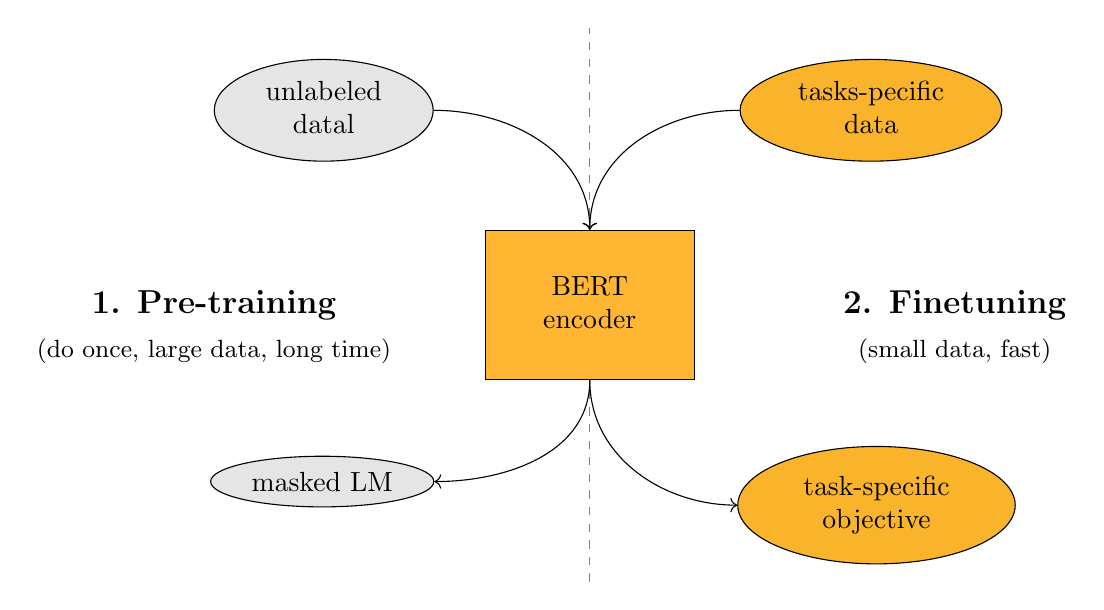
\begin{tikzpicture}

            \visible<3->{\draw[dashed,Gray] (0, -100pt) -- (0, 100pt);}

            \node[draw,fill=Orange!80,inner sep=15pt] (bert) {\begin{tabular}{c}BERT \\ encoder\end{tabular}};

            \visible<2->{
            \node (pre) [left=50pt of bert.west] {\large\bf 1. Pre-training};
            \node (pre2) [below=0pt of pre.south] {\small (do once, large data, long time)};
            \node[draw,ellipse,inner sep=1pt,fill=Gray!20] (unlabeled) [above left=30pt and 30pt of bert.north west] {\begin{tabular}{c}unlabeled \\ datal\end{tabular}};
            \draw[->] (unlabeled.east) to[out=0,in=90] (bert.north);
            \node[draw,ellipse,inner sep=3pt,fill=Gray!20] (mlm) [below left=30pt and 30pt of bert.south west] {masked LM};
            \draw[->] (bert.south) to[out=270,in=0] (mlm.east);}

            \visible<3->{
            \node (fine) [right=50pt of bert.east] {\large\bf 2. Finetuning};
            \node (fine2) [below=0pt of fine.south] {\small (small data, fast)};
            \node[draw,ellipse,inner sep=1pt,fill=Dandelion] (labeled) [above right=30pt and 30pt of bert.north east] {\begin{tabular}{c}tasks-pecific \\ data\end{tabular}};
            \draw[->] (labeled.west) to[out=180,in=90] (bert.north);
            \node[draw,ellipse,inner sep=3pt,fill=Dandelion] (loss) [below right=30pt and 30pt of bert.south east] {\begin{tabular}{c}task-specific \\ objective\end{tabular}};
                    \draw[->] (bert.south) to[out=270,in=180] (loss.west);}


    \end{tikzpicture}
\end{frame}

\begin{frame}{Předtrénování: Masked Language Model}

    \centering
    \fbox{\large
    \colorbox{lightgray}{All}
    \colorbox{lightgray}{human}
    \colorbox{lightgray}{being}
    \colorbox{lightgray}{are}
    \colorbox{lightgray}{born}
    \only<1>{\colorbox{lightgray}{free}}%
    \only<2>{\colorbox{GreenYellow}{free}}%
    \only<3>{\colorbox{Rhodamine!30}{\texttt{MASK}}}%
    \only<4>{\colorbox{Dandelion}{hairy}}%
    \only<5->{\colorbox{GreenYellow}{free}}
    \colorbox{lightgray}{and}
    \colorbox{lightgray}{equal}
    \colorbox{lightgray}{in}
    \colorbox{lightgray}{dignity}
    \colorbox{lightgray}{and}
    \colorbox{lightgray}{rights}}

    \vspace{20pt}

    \begin{enumerate}

        \item<2-> Randomly sample a word $\rightarrow$
            \colorbox{GreenYellow}{free}

        \item<3-> With 80\% change replace with special
            \colorbox{Rhodamine!30}{\texttt{MASK}} token.

        \item<4-> With 10\% change replace with random token $\rightarrow$
            \colorbox{Dandelion}{hairy}

        \item<5-> With 10\% change keep as is $\rightarrow$
            \colorbox{GreenYellow}{free}

    \end{enumerate}

		\vspace{10pt}

    \visible<6->{
    Then a classifier should predict the missing/replaced word
            \colorbox{GreenYellow}{free}}

\end{frame}

% - - - - - - - - - - - - - - - - - - - - - - - - - - - - - - - - - - - - - - -

% ----------------------------------------------------------------------------

\begin{frame}{GPT and few shot learning}

\end{frame}

% ----------------------------------------------------------------------------


\begin{frame}{Férovost dat}

Ukázat sprosťárny a nekorektní kecy, které GPT vygeneruje

\end{frame}


\section{Zpětnovazebné učení}

% ----------------------------------------------------------------------------

\section{Generativní adversariální sítě}


\summary{Shrnutí}{%
    \begin{enumerate}
        \item Advantages of unsupervised methods.
    \end{enumerate}
}
% ----------------------------------------------------------------------------

%}

%\begin{frame}[allowframebreaks]
%\frametitle{Odkazy}
%\bibliographystyle{plainnat}

%\bibliography{odkazy.bib}

%\end{frame}

%\begin{frame}
%\frametitle{References}
%\renewcommand*{\bibfont}{\footnotesize}
%\printbibliography[heading=none]
%\end{frame}


\end{document}
